\section{Logistic Regression}

\textbf{For the linear classification model, we assumed the class-conditional distributions to be Gaussian}
\begin{itemize}
\item We assumed $x| (t=1) \sim \mathcal{N}(\mu_+, \Sigma_+)$ and $x| (t=-1) \sim \mathcal{N}(\mu_-, \Sigma_-)$, and two class-probabilities $P(t=1)$ and $P(t=-1)$.
\item  This is called an \emph{generative model}, as we have written down a full joint model over the data. 
\item  We saw that violations of the model assumption can lead to `bad' decision boundaries.
\end{itemize}

\begin{figure}
	\begin{subfigure}[b]{0.45\textwidth}
		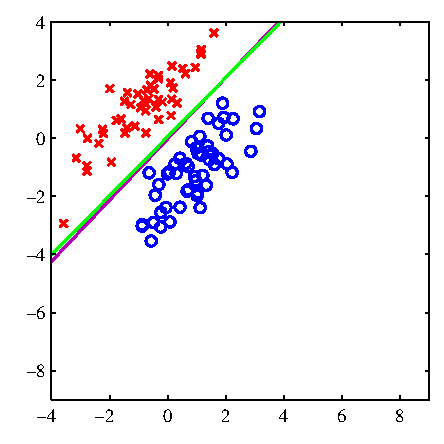
\includegraphics[width=\textwidth]{./lecture7/Figure44a.pdf}
	\end{subfigure}
	~
	\begin{subfigure}[b]{0.45\textwidth}
		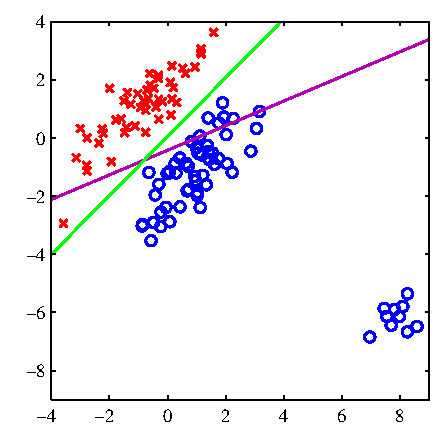
\includegraphics[width=\textwidth]{./lecture7/Figure44b.pdf}
	\end{subfigure}	
	\caption{Figures taken from Bishop PRML}
\end{figure}


\textbf{For regression, we assumed Gaussian outputs, but did not need assumptions about the distribution of inputs.}
\begin{itemize}
\item For linear regression, we conditioned on $x$, and assumed a Gaussian distribution over $t$: $t|x \sim \mathcal{N}(y(x), \gamma^2)$
\item  We maximized the conditional log-likelihood $L(\omega)=\sum_n \log p(t_n|x_n, \omega)$, i.e we assumed that the $x$ were given.
\item  Therefore, this approach to linear regression works for \emph{any} distribution over $x$.
\item $x$ is typically high-dimensional, so it is difficult to make appropriate distributional assumptions for it. 
\end{itemize}

\begin{figure}
	\centering
	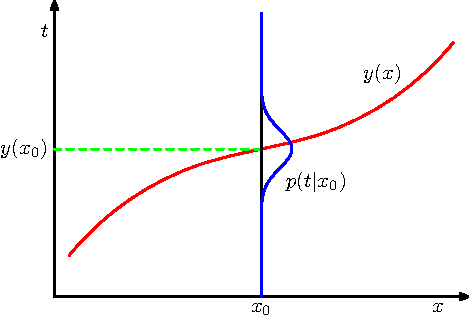
\includegraphics[width=.4\textwidth]{./lecture7/Figure128.pdf}
	\caption{Figure taken from Bishop PRML}
\end{figure}


\textbf{We can define a discriminative model for classification by modelling the conditional class probabilities.}
\begin{itemize}
\item From the homework-exercise, we know that $P(t=1 | z(x))=\sigma(z(x))$ where $\sigma(z)=1/(1+\exp(-z))$ and $z(x)=
\omega^\top x+\omega_o$.
\item Notation is simpler if we use $0$ and $1$ as class labels, so we define $s_n=1$ as the label for the positive class, and $s_n=0$ als label for the negative class.
\item In other words, $s |x \sim \mbox{Bernoulli}(\sigma(z(x))$.
\item Also, we set $y_n=\sigma(z(x))$.
\item  The parameters of $z(x)=\omega^\top x+ \omega_o$ can be learned by maximizing the conditional log-likelihood $L(\omega)=\sum_n \log p(t_n|x_n, \omega)$ [on board]
\item  This is an \emph{discriminative} approach to classification, as we only model the labels, and not the inputs.
\item 
 Decision rule and function shape of $p(t|x)$ will be the same for the generative (`Linear Discriminant Analysis') and the discriminative model, but the parameters were obtained differently.
\end{itemize}

\begin{bbbox}{Log-likelihood for logistic regression}
	Please note that we drop $\omega_0$ for simplicity, or similarly $\omega_0 = 0$.
	\begin{flalign*}
		& z(x) = \omega^{\top}x & \\
		& P\left(\lbrace t_n \rbrace, \lbrace x_n \rbrace, \omega \right) = \prod_{n=1}^N P(t_n|x_n,\omega) & \\
		& \qquad {} = \prod_{n=1}^N \left\{
				\begin{aligned}
		         	& \sigma(z(x)); & t_n = 1; & s_n = 1\\
		         	&1-\sigma(z(x)); & t_n = -1; & s_n = 0
         		\end{aligned} \right. &\\
		& \qquad {} = \prod_{n=1}^N \left\{
				\begin{aligned}
		         	& y_n; & t_n = 1; & s_n = 1\\
		         	& 1-y_n; & t_n = -1; & s_n = 0
         		\end{aligned} \right. &\\
		& \qquad {} = \prod_{n=1}^N y_n^{s_n} (1-y_n)^{1-s_n} \\
		& L_\omega = \sum_{n=1}^N \log \left( p(t_n|x_n,\omega) \right) &\\
		& \qquad {} = \sum_{n=1}^N s_n \log \left( y_n \right) + (1-s_n) \log \left( 1- y_n \right)&\\		
	\end{flalign*}
\end{bbbox}

\subsection{Maximum likelihood estimation of Logistic Regression}

\textbf{Maximum likelihood estimation of Logistic Regression}

\begin{itemize}
\item This algorithm is called \emph{logistic regression}, and is a \emph{much} better algorithm than the algorithms we discussed last week.
\item Need to optimize log-likelihood numerically.
\item  People typically minimize the negative log-likelihood $\mathcal{L}$ rather than maximize the log-likelihood...
\item  To numerically minimize the negative log-likelihood, we need its gradient (and maybe its hessian) [on board]
\end{itemize}

\begin{bbbox}{Gradient and Hessian for Logistic Regression}
	Rather than maximizing the log-likelihood L people usually minimize the negative log-likelihood $\mathcal{L}$. Since there is no close form solution for finding the minimum in the case of a logistic regression we utilize iterative algorithms. Those algorithms require that we calculate the gradient of $\mathcal{L}$: \\
	\begin{flalign*}
		& \frac{\partial \mathcal{L}}{\partial \omega_i}
		    = - \sum_{n=1}^N s_n \frac{1}{y_n} y_n (1-y_n) x_n^{(i)}
		      + (1-s_n) \frac{1}{1-y_n} y_n (-1) x_n^{(i)} & \\
		& \qquad {} = - \sum_{n=1}^N x_n^{(i)} \left[ s_n - s_ny_n - y_n + s_ny_n \right] & \\
		& \qquad {} = \sum_{n=1}^N \left[ y_n -s_n \right] x_n^{(i)} & \\
		& \nabla \mathcal{L} = \sum_{n=1}^N \left[ y_n -s_n \right] x_n & \\
	\end{flalign*}
However some algorithms utilize the so called Hessian of our negative log-likelihood to reduce the number of iterations need for convergence. In word the Hessian is a square matrix of second order partial derivatives of $\mathcal{L}$. Since we have already calculated the first order derivative we can use it to find the Hessian: \\
\begin{flalign*}
	& \frac{\partial \mathcal{L}}{\partial \omega_i \partial \omega_j}
		= \frac{\partial}{\partial \omega_j} \left[ \frac{\partial \mathcal{L}}{\partial \omega_i} \right]
		= \frac{\partial \sum_{n=1}^N \left[ y_n -s_n \right] x_n^{(i)}}{\partial \omega_j}
		= \sum_{n=1}^N \left[ y_n (1- y_n) \right] x_n^{(i)}x_n^{(j)} & \\
	& \nabla \nabla \mathcal{L} = \sum_{n=1}^N \left[ y_n (1- y_n) \right] x_n x_n^{\top} & \\
	& \text{where } \left[x_n x_n^{\top} \right]_{ij} = x_n^{(i)}x_n^{(j)} &
\end{flalign*}
\end{bbbox}

\textbf{The cost-function for logistic regression is convex.}
\begin{figure}
	\begin{subfigure}[b]{0.45\textwidth}
		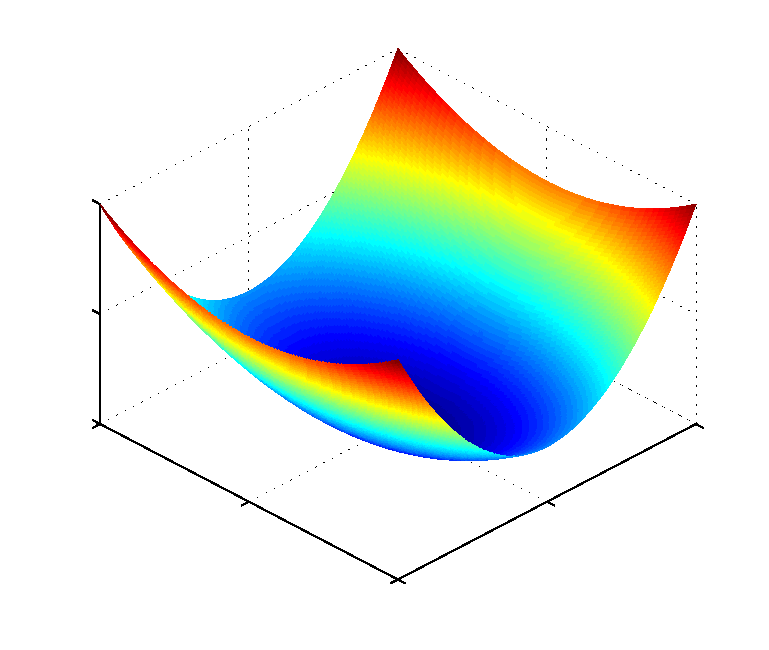
\includegraphics[width=\textwidth]{./lecture7/Convex.pdf}
	\end{subfigure}
	~
	\begin{subfigure}[b]{0.45\textwidth}
		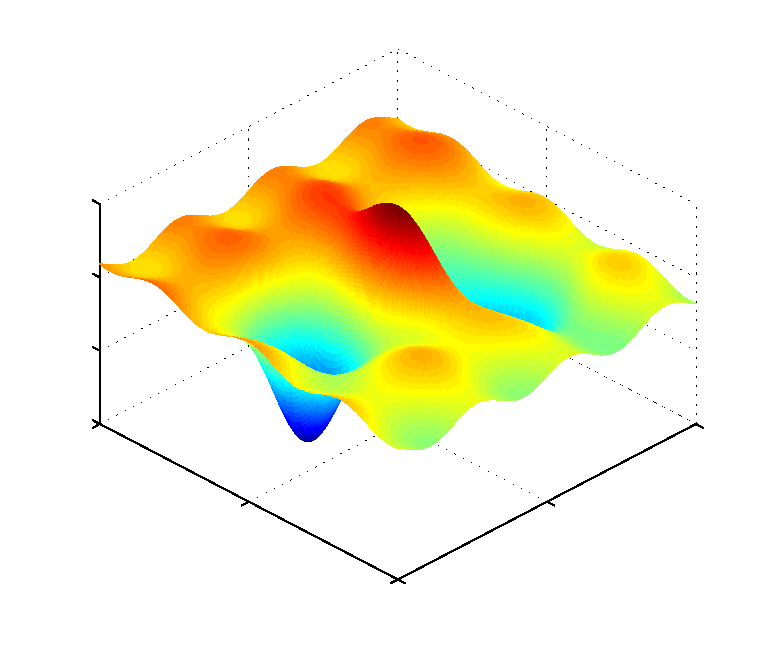
\includegraphics[width=\textwidth]{./lecture7/NotConvex.pdf}
	\end{subfigure}	
\end{figure}

\begin{itemize}
\item  Fact: The negative log-likelihood is \emph{convex} -- this makes life much more easier. 
\item  There are no local minima to get stuck in, and there is good optimization techniques for convex problems. 
\end{itemize}

\begin{bbbox}{Notes on convex functions and the Hessian}
	A function is convex whenever it's Hessian is positive definite.\\
	A matrix is positive definite if: $v^{\top} M v > 0; \forall v: \|v\| \not= 0$ \\
	Note that having a symmetric matrix is not sufficient for a positive definite matrix. \\
	A convex funcion has only one minimum, i.e. minimizing guartuees global minimum.
\end{bbbox}

\textbf{\emph{Gradient descent} is a simple method for numerically minimizing a function.}
\begin{itemize}
\item The gradient $\nabla \mathcal{L}$ of a function points into the direction of steepest descent.
\item  Gradient descent: 'run down the gradient' $\omega_{new}=\omega_{old}-\alpha \nabla \mathcal{L}_\omega$, with learning rate $\alpha$.
\item  Slightly more sophisticated version: numerically optimize $\alpha$ for each step by doing a \emph{line search}.
\item  Convergence can be very slow if cost-function has `valleys'.
\end{itemize}

\begin{figure}
\centering
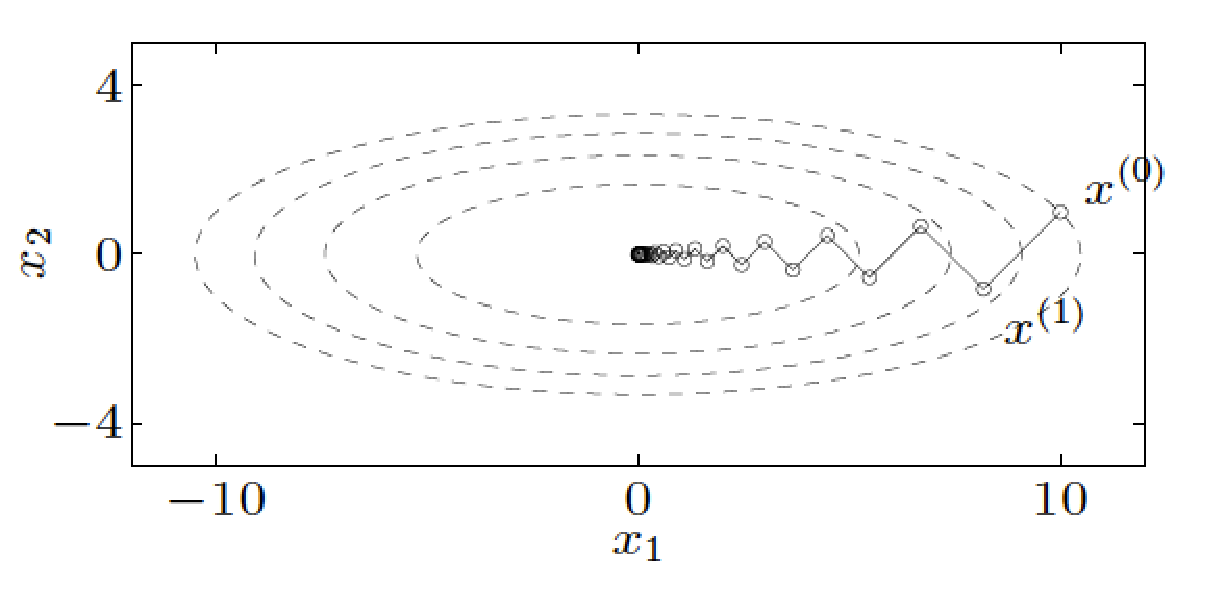
\includegraphics[width=.7\textwidth]{./lecture7/BoydGradientDescent}
\caption{Figure taken from Boyd, Convex Optimization}
\end{figure}

\begin{figure}
	\begin{subfigure}[b]{0.2\textwidth}
		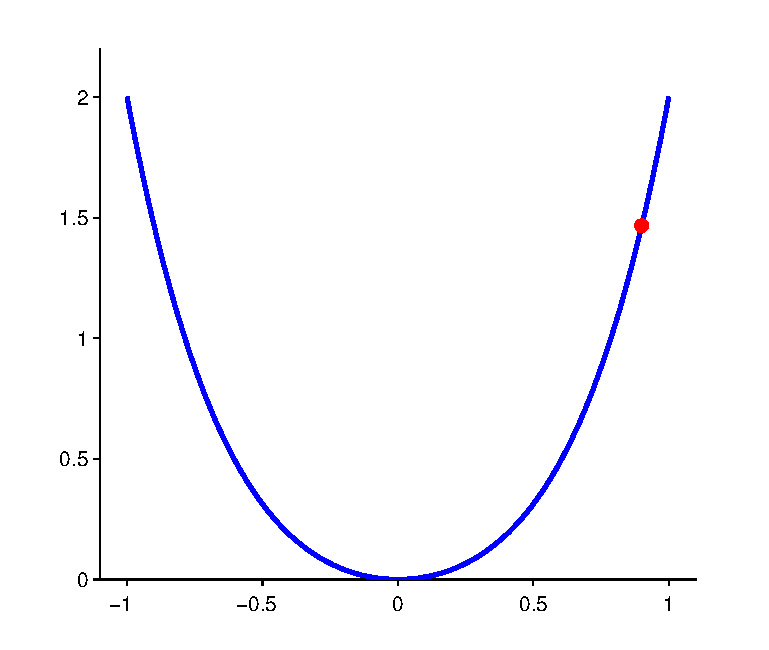
\includegraphics[width=\textwidth]{./lecture7/Newton0}
	\end{subfigure}
	~
	\begin{subfigure}[b]{0.2\textwidth}
		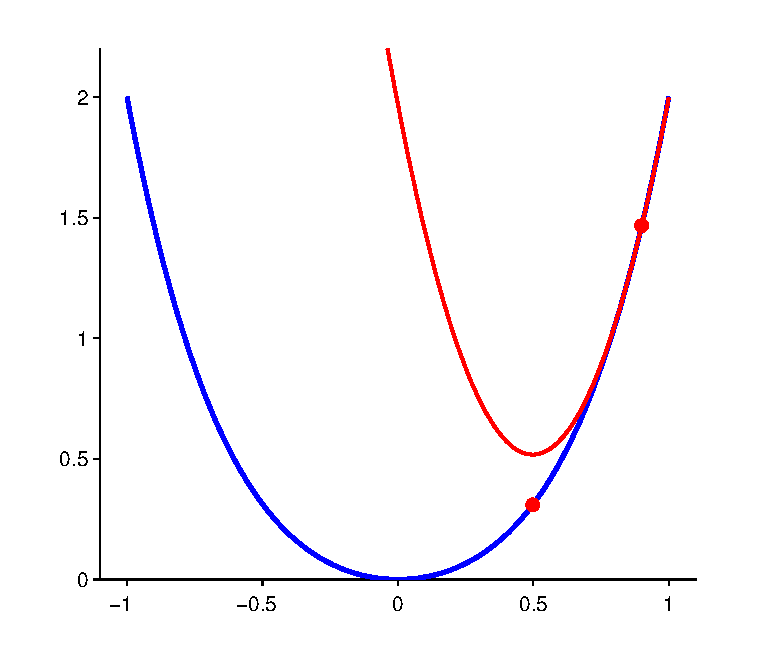
\includegraphics[width=\textwidth]{./lecture7/Newton1}
	\end{subfigure}
	~
	\begin{subfigure}[b]{0.2\textwidth}
		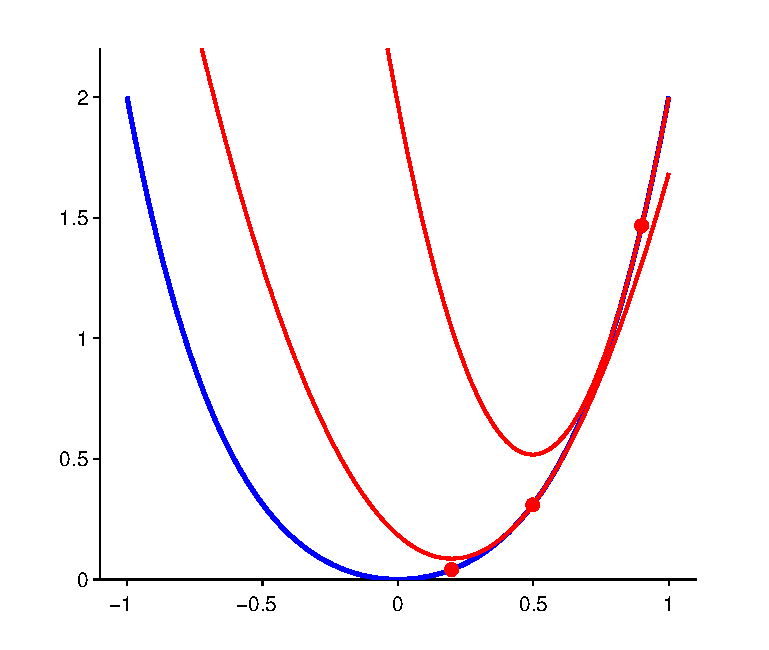
\includegraphics[width=\textwidth]{./lecture7/Newton2}
	\end{subfigure}
	~
	\begin{subfigure}[b]{0.2\textwidth}
		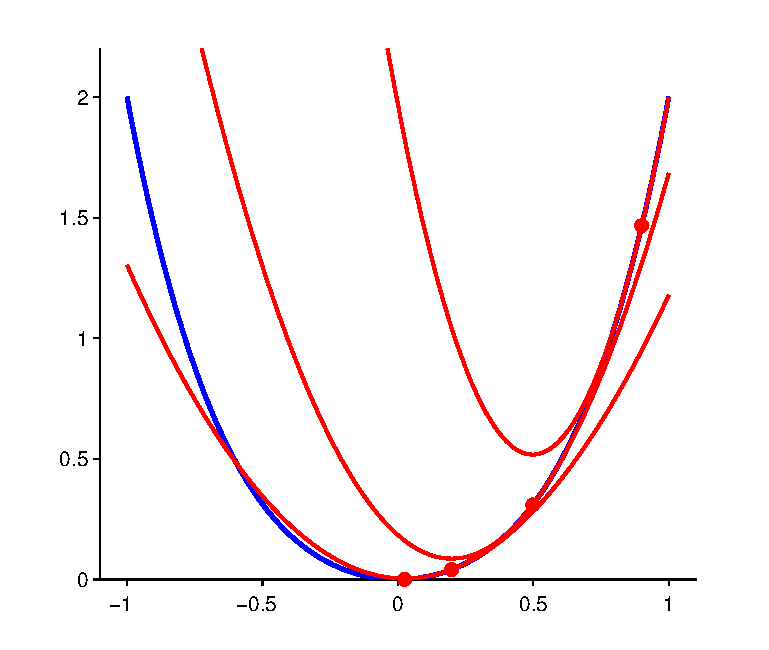
\includegraphics[width=\textwidth]{./lecture7/Newton3}
	\end{subfigure}
	\\
	\begin{subfigure}[b]{0.2\textwidth}
		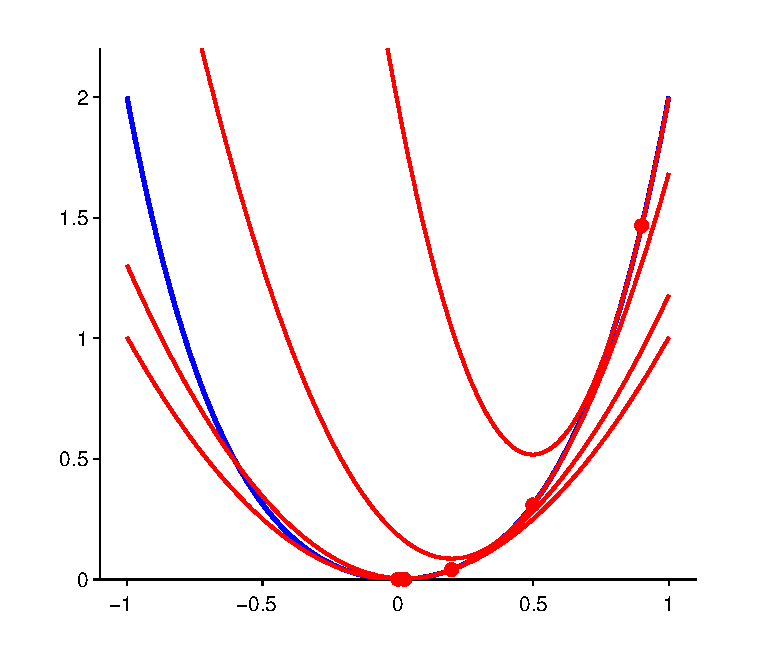
\includegraphics[width=\textwidth]{./lecture7/Newton4}
	\end{subfigure}
	~
	\begin{subfigure}[b]{0.2\textwidth}
		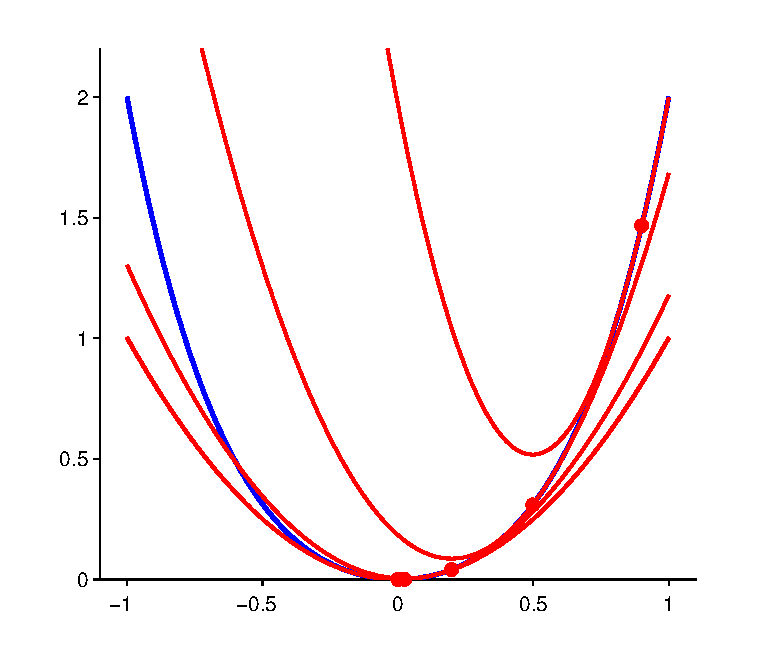
\includegraphics[width=\textwidth]{./lecture7/Newton5}
	\end{subfigure}
	~
	\begin{subfigure}[b]{0.2\textwidth}
		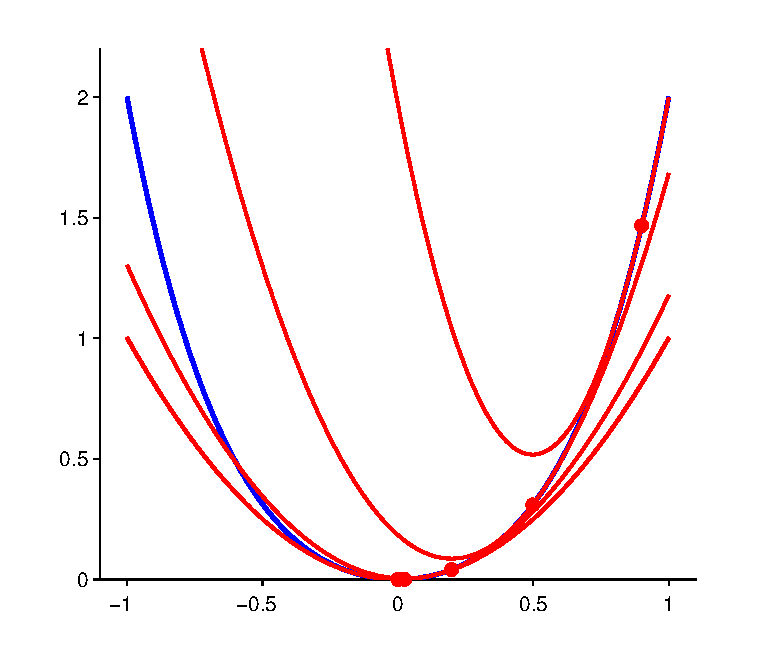
\includegraphics[width=\textwidth]{./lecture7/Newton6}
	\end{subfigure}
	\caption{\emph{Iterative Least Squares:} Approximate by parabola, minimze, iterate.}
\end{figure}



\textbf{\emph{Iterative Least Squares} is a more efficient method for minimizing the cost-function}
\begin{itemize}
\item Newton-Raphson: $\omega_{new}=\omega_{old}-\alpha (\nabla \nabla \mathcal{L})^{-1}\nabla L_\omega$ 
\item Pre-multiplying the gradient by the inverse-hessian speeds up convergence `along valleys' (analogy with LDA)
 \item Motivation: For quadratic functions $F(x)=a+b^\top x+ x^\top B x$, Newton-Raphson finds the minimum in one iteration.
 \item In this contex, Newton-Raphson (with $\alpha=1$) is often called \emph{iterative least squares}.
 \item Note: Newtwn's method can be bad if problem is not convex, and can be slow if it is difficult to calculate/invert the Hessian. A large number of optimization algorithms exist which do not require the (complete) Hessian (quasi Newton/BFGS, etc..). 
% \item Any (reasonable) optimization algorithm requires the gradient.
\end{itemize}


\textbf{Visualizing the cost-function of logistic regression}

[on board]


\subsection{Bayesian Logistic Regression: Approximating the posterior distribution}
\textbf{Bayesian inference for this model does not have a closed form solution}
\begin{itemize}
\item Typically use Gaussian prior on $\omega$.
\item For linear regression, posterior distribution was Gaussian, with closed-form solutions for the mean and covariance.
\item For logistic regression, the posterior distribution is non-Gaussian.
\item  Popular approximation: Approximate posterior by a Gaussian
\begin{align}
p(\omega|D) \approx \mathcal{N}(\mu_{post}, \Sigma_{post})
\end{align}
\item  Different methods exist for finding `good' $\mu_{post}$ and $\Sigma_{post}$: Expectation Propagation (EP), Laplace Approximation, Variational Inference
\end{itemize}

\textbf{The Laplace-Approximation is a simple Gaussian approximation to the posterior}
\begin{itemize}
\item \emph{Laplace approximation:} $\mu_{post}=\omega_{MAP}$, $\Sigma_{post}=\left(\nabla \nabla_\omega L   \right)^{-1}$. 
\item Take MAP as mean, and inverse hessian at MAP as covariance.
\item  Motivation: Curvature matching, Taylor-expansion [on board]
\item  Q: When will the Laplace approximation fail?
\end{itemize}
\begin{figure}
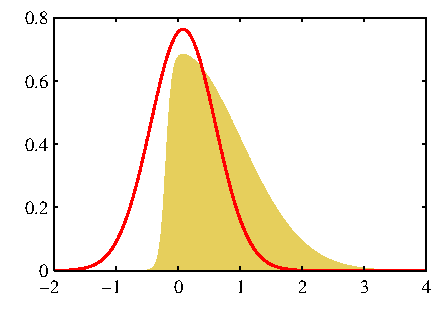
\includegraphics[width=.49\textwidth]{./lecture7/Figure414a.pdf}
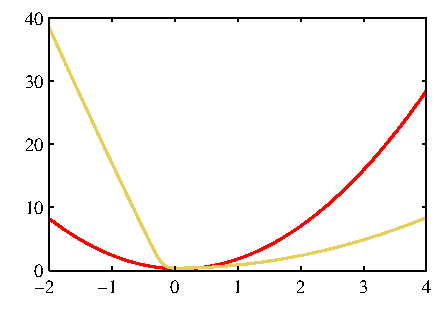
\includegraphics[width=.49\textwidth]{./lecture7/Figure414b.pdf}
\caption{Figure taken from Bishop PRML}
\end{figure}

%\textbf{The posterior distribution can be used to calculate the predictive distribution and to optimze hyper-parameters}
%[on board]

%\section{LR's popular little brother-- support vector machines}

%\section{The exam}